\section{Photon beam flux  \label{sec:flux}   }

\subsection{Photon beam flux accounting with the GlueX pair spectrometer}
The photon beam flux can be directly extracted by analyzing the Pair Spectrometer (PS) data. There is a thin beryllium converter installed in
the beam upstream of the PS to produce electron-position pairs.
The absolute normalization of the PS
is performed with the Total Absorption Counter (TAC) during dedicated
runs.

The systematics of the photon beam flux accounting using the pair
spectrometer originates from a few main contributions: the overall
quality of the spectrometer calibration using the TAC; the accuracy
of the Monte Carlo
simulation of this process; long-term stability of the performance of the
pair spectrometer; and possible changes of beam conditions between
low-intensity running (necessary for the TAC
calibration) and production intensity.  There are a few other
contributions, all less significant. The acceptance of the GlueX PS \cite{hdnote3684} is shown
in Fig.~\ref{fig:psacc}. For the proposed experiment the PS magnetic field
should be reduced to cover the beam energy range of 5-6~GeV.
\begin{figure}[tpb]
\begin{center}
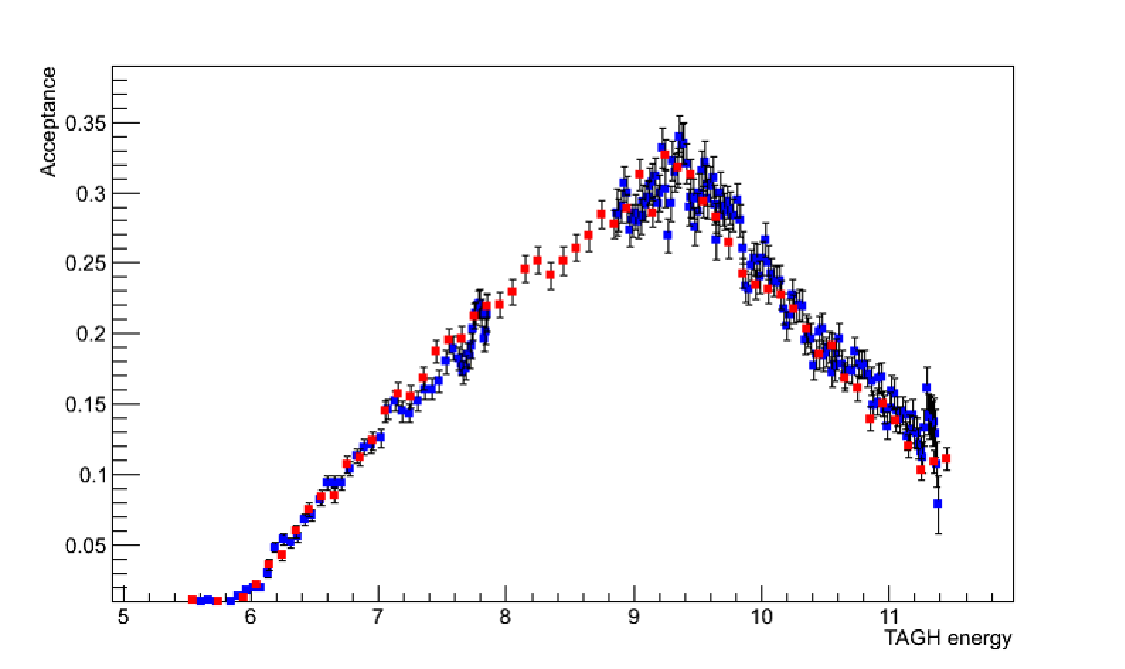
\includegraphics[width=10cm,angle=0]{figures/ps_acceptance.pdf}
\end{center}
\caption{GlueX PS acceptance extracted from TAC data analysis (blue
  points) and Monte Carlo simulation (red points).}
\label{fig:psacc}
\end{figure}
The methodology of the PS analysis is the same as in the
PrimEx-eta experiment, currently running in Hall~D, and has an accuracy
$\sim 1.0$-1.5\% \cite{PrimexDexp}.

\subsection{Cross section verification with the exclusive single $\pi^{0}$ photoproduction  \label{sec:pi0norm} }
The extracted cross section can also be normalized, independently
from a PS analysis, with a simultaneous measurement of the $\pi^0$ radiative decay width.  Fig.~\ref{fig:leaddndt} shows the exclusive single $\pi^0$
photoproduction yield at forward angles obtained by the PrimEx
experiment during its measurement of the width.

The photon beam flux in PrimEx was $0.725\times10^{12}$ for
the 4.9-5.5~GeV portion of a tagged bremsstrahlung beam impinging on
a 5\% radiation length lead
target. The distance between the calorimeter and target was 7.3~m
and the central square part of the calorimeter used in the analysis was
$70\times70$~cm. These conditions are to be compared with the
proposed NPP experimental conditions. We seek 20 days of $10^7$ photons per second from a tagged, collimated coherent bremsstrahlung beam
(i.e., 20 times more than the PrimEx lead target beam flux), the
distance between the target and FCAL is 6.2~m and the active region of
the calorimeter has a diameter of 2~m.
The central hole for
PrimEx was $8\times8$~cm and for FCAL $20\times20$~cm, where
in both cases it is assumed that the innermost layer of crystals/blocks
are excluded from the analysis. This is a relative decrease in
acceptance at forward angles for the FCAL.
This comparison leads us to expect an order of
magnitude higher statistics for exclusive single
$\pi^0$ photoproduction for NPP compared to PrimEx.
Thus the PrimEx statistical uncertainty for lead will decrease from
2.5\% down to 1.0\%.\footnote{Note that this is only
the portion of the statistics that PrimEx
obtained on a lead target.} The systematic uncertainty
in PrimEx was 2.1\% and had two major contributions: yield
extraction (1.6\%) and photon beam flux accounting
(1.0\%).  The first contribution is partly statistically
driven, and would have been smaller with increased statistics,
and the second one cancels in the comparison with the proposed experiment
since it is the same photon beam flux for the single and double exclusive
$\pi^0$ photoproduction. The main factors increasing
systematics for the NPP experiment are: the angular resolution of FCAL is about a factor of two worse than for
the lead tungstate crystals used in PrimEx
%the single $\pi^0$ photoproduction theory needs to be involved since
%the photon beam energy spectra are not the same for PrimEx and
%proposed experiment;
and there is no dipole magnetic downstream of the target to sweep out
charged backgrounds as there was in PrimEx. As a result we can expect
slightly worse systematic
uncertainty than in PrimEx and a statistical precision of 1.0\%,
i.e., a total error 2.5-3.5\% for the $\pi^0$ radiative width, where uncertainties due to the absolute photon beam flux accounting,
the number of target atoms,
and FCAL trigger efficiency all largely cancel.
The expected total
uncertainty for such a normalization needs to include the PrimEx
total error of the $\pi^0$ radiative width, which was recently
reported as 1.5\% \cite{Larin:2018}.  All this gives a 3-4\%
error for cross section normalization via re-extracting the $\pi^0$
radiative decay width.

\subsection{Muon pair production}
In addition to these normalization channels, production of muon pairs,
which has a known cross section, can be used as a measurement of
photon flux. Since the experiment will be running concurrently with
the Charged Pion Polarizability (CPP) experiment, the photon flux on
target will be the same. CPP plans to use muon pair
creation by beam photons as its main normalization channel, and so
those measurements will be available for normalization of the neutral
pion channel as well. In the case of CPP, the GlueX track finding and
fitting efficiency will have to be determined for muon pairs, but any
systematic error in that determination will largely cancel when
applied to the charged pion pairs of interest for CPP.
That will not be the case for the
neutral pion channel and this will have to be taken into account when
evaluating systematic errors using this method of normalization. In
any case, muon pair production should provide a useful check on the
other methods described above.
